% =====================================================================
%  RESULTADOS
%  Cifras de RESULTADOS_OE4_SIMULACION.md y de la evidencia de hardware
%  S24_peldano2 / S24_nav2_navegacion / S25_pisos34_campo /
%  S26_piso4_cadena_media_vuelta / S26_piso3_deepy_y_saturacion.
%
%  2026-10-15: escrito para el lector de la tesis, sin códigos del
%  repositorio (compuertas, requisitos, condiciones A/B), sin «§» y sin
%  fechas de bitácora. Las tres cosas que hay que escribir con cuidado van
%  en la sección de limitaciones: la continuidad es un invariante; el
%  intervalo de Wilson sostiene «supera el 70 %», no «es del 86,7 %»; y la
%  campaña corrió con un mapa que leía libre lo desconocido.
% =====================================================================
\chapter{Resultados}
\label{cap:resultados}

\begin{notaavance}[la toma de datos cierra el 16 de octubre de 2026]
Las dos partes de este capítulo están en situaciones distintas. La
sección~\ref{sec:res-sim}, de simulación, está cerrada: la campaña de treinta
misiones fue dictaminada válida y sus números no van a cambiar. La
sección~\ref{sec:res-hw}, con los vehículos, va por partes. La odometría y la
navegación de un vehículo superaron sus pruebas de verificación y se reportan. La
misión con relevo entre los dos vehículos y la campaña con los vehículos se
corren el 16 de octubre, y la sección~\ref{sec:res-completo} queda sin redactar
hasta entonces. Después de esa fecha no se toman más datos.
\end{notaavance}

Los resultados llegan de dos campañas distintas. La primera, en simulación, con
treinta misiones sorteadas. La segunda, sobre los vehículos reales en los
pasillos del edificio. Se reportan por separado porque miden aspectos distintos:
la de simulación mide el sistema completo con relevo, y la de los vehículos mide
hasta dónde llega la plataforma física.

% ---------------------------------------------------------------------
\section{Evaluación en simulación}
\label{sec:res-sim}

La campaña corrió treinta misiones sorteadas: quince de control, con origen y
destino en el mismo piso, y quince entre pisos, con un relevo. El analizador la
dictaminó válida, sin ningún descarte, frente a un máximo admitido del 20~\%.

\subsection{Tasa de éxito}

Una misión es exitosa si cumple dos condiciones. La primera, que la pose final
quede a 0,25~m o menos del destino, medida contra la odometría y no contra el
resultado de Nav2. La segunda, que la misión llegue a completarse sin pasar por
fallo. La tabla~\ref{tab:exito} da la tasa de cada grupo con su intervalo de
confianza de Wilson al 95~\% \autocite{wilson1927probable}.

\begin{table}[H]
  \centering\small
  \caption{Tasa de éxito de la campaña en simulación, con intervalo de confianza
    de Wilson al 95~\%.}
  \label{tab:exito}
  \begin{tabular}{@{}lcccc@{}}
    \toprule
    \textbf{Misiones} & \textbf{n} & \textbf{éxitos} & \textbf{tasa} & \textbf{intervalo al 95~\%} \\ \midrule
    Campaña completa & 30 & 26 & 86,7 \% & 70,3 -- 94,7 \% \\
    Mismo piso (control) & 15 & 12 & 80,0 \% & 54,8 -- 93,0 \% \\
    Entre pisos, con relevo & 15 & 14 & 93,3 \% & 70,2 -- 98,8 \% \\ \bottomrule
  \end{tabular}
\end{table}

Lo que se puede afirmar es que la tasa de éxito supera el 70~\%, no que sea del
86,7~\%. Con treinta misiones el intervalo mide 24 puntos porcentuales de ancho,
y ese límite es de diseño: solo se reduce con más muestra. El 86,7~\% es el
estimador puntual y se reporta siempre junto a su intervalo.

Los intervalos de los dos grupos se solapan, así que la comparación entre ellos
no sostiene ninguna conclusión. Conviene decirlo porque el estimador puntual
apunta en contra de la intuición: las misiones con relevo salieron mejor que las
de control.

\subsection{Causa común de los cuatro fallos}

Las cuatro misiones fallidas quedaron a 0,295, 0,284, 0,311 y 0,347~m del
destino, frente a una tolerancia de 0,25~m. Las cuatro se quedaron cortas:
ninguna se pasó del destino ni terminó en otro sitio. Los cuatro fallos se deben
al límite de precisión de la aproximación final, y ninguno a la coordinación. El
error de llegada del conjunto tiene una mediana de 0,106~m y va de 0,019 a
0,347~m.

\subsection{Tiempo de respuesta y tiempo de asignación}

El tiempo de respuesta se reporta por escalones, y no con media y desviación, por
una razón de instrumento (tabla~\ref{tab:respuesta}).

\begin{table}[H]
  \centering\small
  \caption{Tiempo de respuesta de las treinta misiones, en escalones del reloj de
    la simulación.}
  \label{tab:respuesta}
  \begin{tabular}{@{}lcccc@{}}
    \toprule
    \textbf{Tiempo de respuesta} & 0,1 s & 0,2 s & 0,3 s & 0,4 s \\ \midrule
    Misiones & 10 & 15 & 4 & 1 \\ \bottomrule
  \end{tabular}
\end{table}

Los cuatro valores son múltiplos exactos de 100~ms, que es el paso con que avanza
el reloj de la simulación. La resolución del instrumento vale entre el 25~\% y el
100~\% de la magnitud medida. Una mediana de 0,2~s significa «uno o dos pasos del
reloj», no «doscientos milisegundos», y dar media y desviación sugeriría una
precisión que el reloj no entrega. Lo que sí se sostiene es la cota, que además es
lo que le importa a un usuario: el robot arranca en menos de medio segundo.

El tiempo de asignación quedó por debajo de 100~ms en las treinta misiones, varios
órdenes de magnitud por debajo de un paso del reloj. Por eso se caracterizó
aparte, en un banco de pruebas con el reloj del sistema: mediana entre 154 y
175~\textmu s y máximo de 306~\textmu s.

\begin{figure}[H]
  \centering
  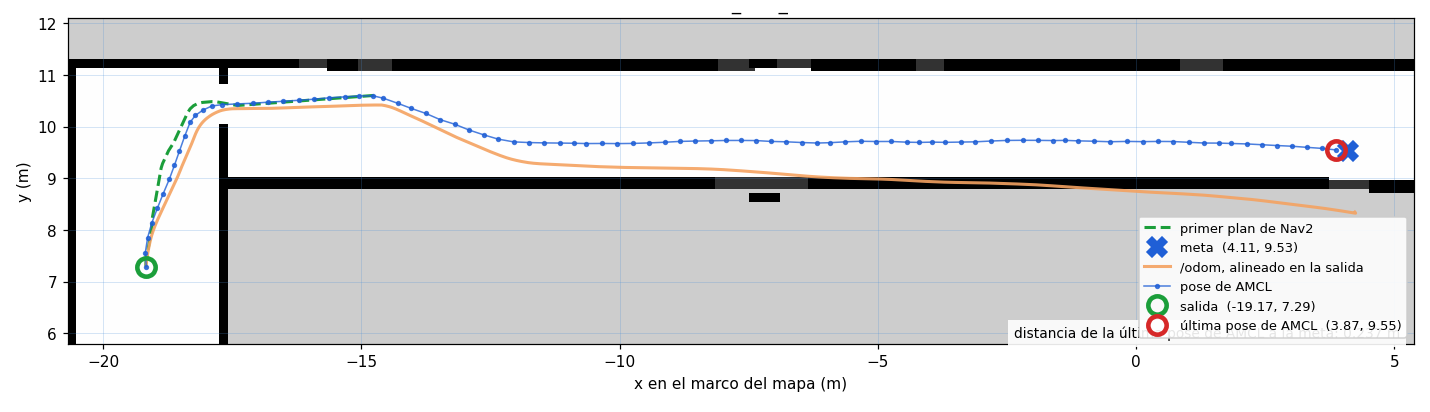
\includegraphics[width=\textwidth]{imagenes/corrida_simulacion.png}
  \caption{Una misión de la campaña en simulación. Se superponen el primer plan
    que calcula el navegador, la pose estimada a lo largo del recorrido y la
    odometría cruda. La separación creciente entre las dos últimas es la deriva
    que la localización corrige contra el mapa.}
  \label{fig:simulacion}
\end{figure}

% ---------------------------------------------------------------------
\section{Evaluación con los vehículos}
\label{sec:res-hw}

La demostración física se organizó en pruebas de verificación sucesivas
(sección~\ref{sec:pruebas-verificacion}). Esta sección reporta las que se han
superado y que producen cifras: la de odometría y la de navegación de un
vehículo.

\subsection{La odometría del vehículo}

El vehículo no tiene codificadores en las ruedas, así que su odometría sale de
comparar barridos sucesivos del láser. Durante meses esa pieza no produjo una
medida utilizable. La tabla~\ref{tab:odometria} reúne lo que se midió en cada
entorno, como fracción del avance real medido con flexómetro.

\begin{table}[H]
  \centering\small
  \caption{Fracción del avance real que registra la odometría, por entorno. El
    criterio de la prueba es un error de 10~\% o menos.}
  \label{tab:odometria}
  \begin{tabular}{@{}lccl@{}}
    \toprule
    \textbf{Entorno} & \textbf{Recorrido} & \textbf{Registrado} & \textbf{Criterio} \\ \midrule
    Pasillo simulado, 46,9 m & largo & 37,9 \% & no cumple \\
    Pasillos de los pisos 1 y 2 & largo & 5,7 \% y 1,3 \% & no cumple \\
    Hall del piso 2 & 6 m & 73 \% & no cumple \\
    Cuarto cerrado, desplazado a mano & 3 m & 96,3 -- 101,9 \% & cumple \\
    Pasillo del piso 4 & 6,68 m & 95,4 \% & cumple \\
    Pasillo del piso 4 & 14,57 m & 103,3 \% & cumple \\
    Pasillo del piso 4, con la unidad inercial & 8,08 m & 101,9 \% & cumple \\
    Pasillo del piso 4, con la unidad inercial & 2,82 m & 104,9 \% & cumple \\ \bottomrule
  \end{tabular}
\end{table}

El estimador es el mismo en todas las filas; lo que cambió fue el entorno. En un
pasillo recto y uniforme la información de avance no está en la señal del
sensor, y ningún ajuste la recupera (sección~\ref{sec:teo-localizacion}). En un
pasillo con hornacinas, casilleros y quiebres, con ocho cambios de perfil en
25~m, la misma odometría queda dentro del $\pm$5~\% sin cambiar un parámetro.

Con las dos mediciones del pasillo del piso 4, de 6,68 y 14,57~m, los directores
dieron por superada la prueba de odometría. Era la condición que el proyecto
venía señalando como el paso del que dependía todo lo demás sobre los vehículos.

Las dos últimas filas ya incluyen la unidad inercial (sección~\ref{sec:imu}). El
avance lo estima el filtro, que lo toma de la misma odometría del láser. El
segundo tramo mide 2,82~m, por debajo de los 5~m que pide el criterio, y se
incluye como dato de la misma cadena.

\subsection{La navegación y la precisión de llegada}
\label{sec:res-g3}

La prueba de navegación de un vehículo pide un recorrido de punto a punto con
Nav2 y la llegada verificada con flexómetro, a 0,5~m o menos del destino. Esa es
la tolerancia que fijó el director para los vehículos reales.

En la primera sesión en el piso 4, las dos llegadas medidas quedaron a 0,57 y
0,62~m, cortas. Nav2 daba entonces la meta por alcanzada a 1,0~m, y los dos
vehículos se detuvieron al cruzar ese margen. Con la unidad inercial integrada
(sección~\ref{sec:imu}) el margen bajó a 0,5~m. En la sesión siguiente, uno de los
vehículos recorrió en el piso 4 tres tramos encadenados, sin que nadie lo tocara
entre uno y otro, y después regresó a la salida (tabla~\ref{tab:g3} y
figura~\ref{fig:cadena}).

\begin{table}[H]
  \centering\small
  \caption{Cadena de tres tramos en el piso 4 y regreso a la salida: llegada de
    cada tramo.}
  \label{tab:g3}
  \begin{tabular}{@{}llcccl@{}}
    \toprule
    \textbf{Tramo} & \textbf{Destino} & \textbf{Tiempo} & \textbf{Recuperaciones} & \textbf{A la meta} & \textbf{Medida} \\ \midrule
    1 & Salón 403 & 13,5 s & 1 & 0,26 m & estimada \\
    2 & Salón 402 & 27,8 s & 1 & 0,45 m & flexómetro \\
    3 & Salón 401 & 5,2 s & 0 & 0,06 m & flexómetro \\
    Regreso & Salida & 62,8 s & 6 & 0,34 m & flexómetro \\ \bottomrule
  \end{tabular}
\end{table}

Las llegadas medidas quedaron dentro de la tolerancia de 0,5~m, y los directores
dieron por superada la prueba. La llegada al Salón 403 no se midió porque en ese
momento no había flexómetro, y se estimó con el error de los otros dos tramos. El
regreso a la salida incluyó una media vuelta en el tramo ancho frente a los
salones, que Nav2 resolvió con seis recuperaciones.

\begin{figure}[H]
  \centering
  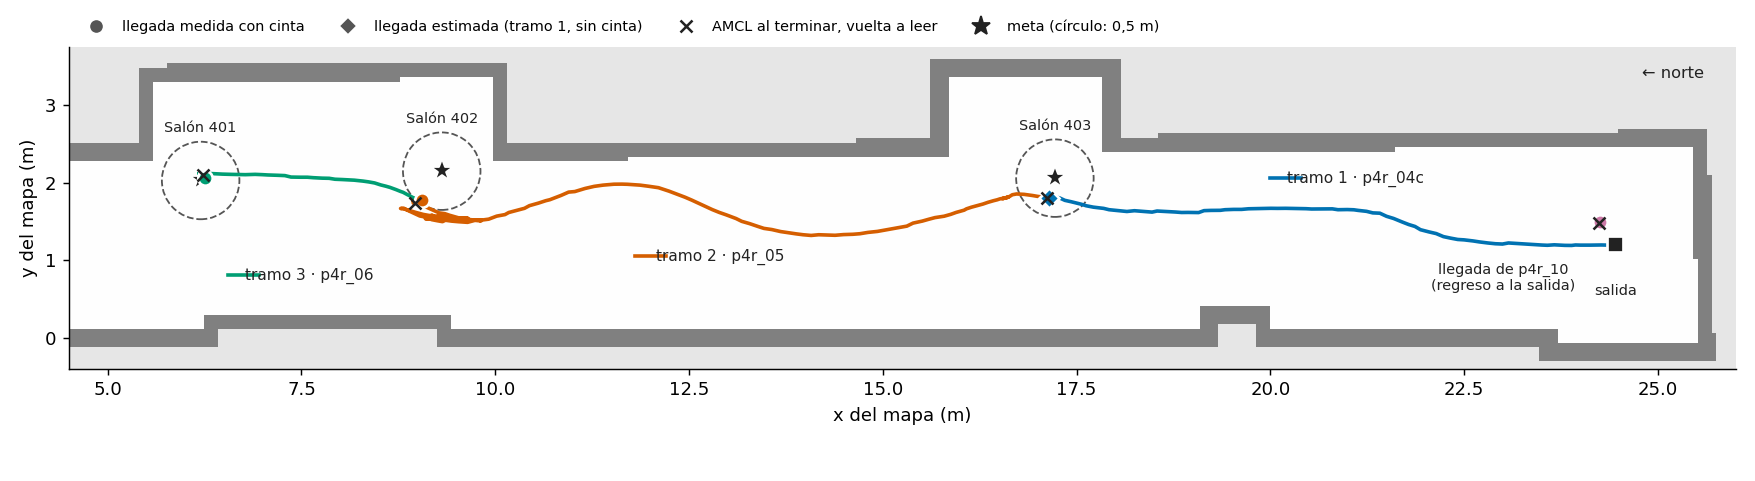
\includegraphics[width=\textwidth]{imagenes/cadena_piso4.png}
  \caption{Cadena de tres tramos en el piso 4 y regreso a la salida: recorrido
    según la localización, llegadas medidas con flexómetro, la llegada estimada
    al Salón 403 y la pose de la localización al terminar cada tramo.}
  \label{fig:cadena}
\end{figure}

Al día siguiente, el otro vehículo recorrió el piso 3 en cinco tramos
encadenados, con dos medias vueltas entre ellos, y los cinco terminaron con éxito
y sin recuperaciones. Esas llegadas no se midieron con flexómetro. Al terminar
cada tramo se forzó a la localización a recalcular su pose, y esta se desplazó
entre 0,61 y 0,86~m. La pose que publica la localización al detenerse el vehículo
va atrasada, y por eso la llegada que vale es la medida con flexómetro.

Lo que condiciona la precisión de llegada sigue siendo la banda muerta de
tracción (sección~\ref{sec:banda-muerta}): el vehículo se aproxima a la meta a
0,40~m/s y no tiene régimen de aproximación fina.

\subsection{El sistema completo con los dos vehículos}
\label{sec:res-completo}

\begin{notaavance}[apartado sin redactar: la toma de datos cierra el 16 de
octubre de 2026]
Aquí irán la misión con relevo entre los dos vehículos, del Salón 302 al Salón
402, y la campaña con los vehículos: diez misiones con relevo entre los pisos 3
y 4, sorteadas antes de correr y ejecutadas sin reubicar los vehículos. Se
reportan con las métricas del protocolo y la tolerancia de 0,5~m, siempre por
separado de la campaña en simulación.
\end{notaavance}

% ---------------------------------------------------------------------
\section{Limitaciones de la medición}
\label{sec:limitaciones}

Tres límites afectan a cómo deben leerse los resultados anteriores. Se declaran
aquí porque callarlos sería presentar como medida lo que no lo es.

\subsection{Naturaleza del criterio de continuidad entre niveles}

La continuidad del servicio es la variable de respuesta principal del cuarto
objetivo, y su criterio binario se cumplió en las treinta misiones. Ese resultado,
sin embargo, no es evidencia, y la razón es estructural.

El criterio exige que, dentro de la ventana de la misión, el coordinador nunca
esté en estado inactivo y nunca tenga el agente sin asignar. Los dos únicos
puntos del código que producen esos valores ocurren antes de que la ventana se
abra. No existe ejecución posible que lo incumpla: son cero incumplimientos de
cero posibles. Un criterio que no puede dar resultado negativo no aporta
evidencia, por muchas veces que se verifique \autocite{popper1959logic}.

La corrección no consistió en inventar una ruta de fallo, que habría sido
instrumentar el experimento para que pareciera más informativo. La continuidad se
declaró como un invariante estructural del diseño. La afirmación se apoyó en una
magnitud que sí varía: el intervalo de tiempo del relevo, entre el final del
tramo de un vehículo y el inicio del tramo del otro. En las quince misiones entre
pisos tuvo una mediana de 0,1~s y un máximo de 0,2~s, es decir, uno o dos pasos
del reloj de la simulación.

\subsection{Ancho del intervalo de confianza}

Ya se dijo con la tabla~\ref{tab:exito}, y se repite porque es el límite más fácil
de olvidar al redactar: con treinta misiones, lo que se puede defender es una cota
inferior, no un valor puntual. Aumentar la confianza exige más muestra.

\subsection{Espacio desconocido marcado como libre en el mapa}

El mapa con que corrió la campaña declaraba un umbral que hacía que 10\,908
celdas desconocidas, el 14,5~\% del mapa, se cargaran como espacio libre. Con
ello quedaban desactivadas en la práctica las dos salvaguardas que debían impedir
planificar sobre lo no explorado.

Esto no invalida el veredicto de la campaña. Los cuatro fallos fueron de
precisión de llegada, no de trazado, y el pasillo por el que se navegó está
mapeado como libre en el mundo real. Lo que no se sabe es si alguna trayectoria
cruzó una de esas celdas, y es comprobable sobre los registros conservados. El
defecto se corrigió después de la campaña.
